\documentclass[12pt]{Qual}
\usepackage{preamble}

\name{Kayla Orlinsky}
\course{Complex Analysis Exam}
\term{Fall 2017}
\hwnum{Fall 2017}

\begin{document}

\begin{problem} $\,$
Let $f(z)=u(z)+iv(z)$ be an entire function and assume that $|u(z)|\ge|v(z)|$ for all $z\in\mathbb{C}.$ Show that $f$ is a constant.
\end{problem}


\begin{solution}$\,$
Clearly $f(\mathbb{C})\subset\{x+iy:|y|\le|x|\}.$ This set can be broken down into the four quadrants to get

\begin{center}
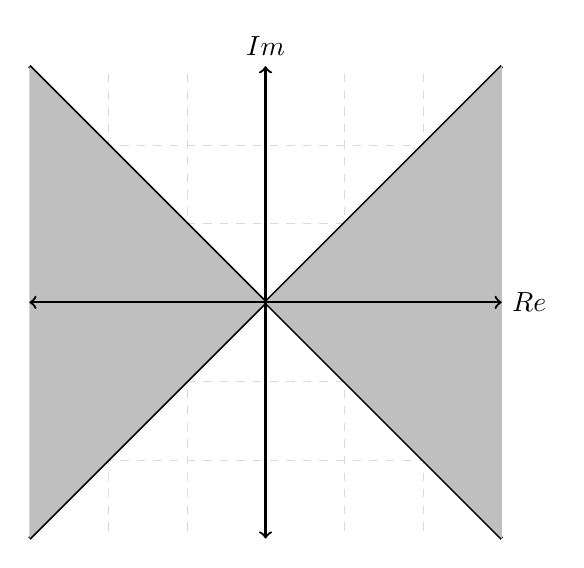
\begin{tikzpicture}
\draw[help lines, color=gray!30, dashed] (-2.9,-2.9) grid (2.9,2.9);
\draw[very thick] (-3,-3) -- (3,3);
\fill[color=gray!50, domain=-3:3, variable=\x]
      (-3, 0)
      -- plot ({\x}, {\x})
      -- (3, 0)
      -- cycle;
\draw[very thick] (-3,3) -- (3,-3);
\fill[color=gray!50, domain=-3:3, variable=\x]
      (-3, 0)
      -- plot ({\x}, {-\x})
      -- (3, 0)
      -- cycle;
\draw[<->, thick] (-3,0)--(3,0) node[right]{$Re$};
\draw[<->, thick] (0,-3)--(0,3) node[above]{$Im$};
\end{tikzpicture}
\end{center}

Now, since $\mathbb{C}$ is open, by the open mapping theorem, $f(\mathbb{C})$ must be open. Therefore, $f(\mathbb{C})$ cannot contain $0$.

Furthermore, $f(\mathbb{C})$ must be connected. Thus, $f(\mathbb{C})$ is either entirely in the left-half plane or entirely in the right-half plane.

WLOG, assume $\re(f(z))>0$ for all $z.$ Namely, that $f$ is contained in the right half plane.

Then, let $g(z)=iz$ and $T(z)=\frac{z-i}{z+i}$.

Then $T\circ g\circ f$ is an entire map from $\mathbb{C}$ to the unit disk $\mathbb{D}$. Therefore, by Louiville's Theorem, $T\circ g\circ f$ is constant.

However, this forces $f$ to be constant since $g$ and $T$ certainly are not constant.
\end{solution}
\newpage



\begin{problem} $\,$
Let $\alpha\in(0,1)$ and $n\in\mathbb{N}$. Prove that the equation $e^z(z-1)^n=\alpha$ has exactly $n$ \textit{simple} roots in the right half plane $\{z:\re(z)>0\}.$
\end{problem}

\begin{solution}$\,$
This problem is nearly identical to \textbf{Spring 2016: Problem 2}, with the only difference being that the root is now a real number.

First, we note that if $e^z(z-1)^n=\alpha$ and $z$ is in the right half plane, then $\re(z)\ge0$ so $|e^z|\ge1$. Namely, \begin{align*}
    |z-1|^n&\le|e^z||z-1|^n\\
    &=|\alpha|\\
    &<1
\end{align*}

Thus, $|z-1|<1$ and so the roots that lie in the right half plane are all contained in the circle $\{|z-1|<1\}.$

Now, let $f(z)=e^z(z-1)^n-\alpha$ and $g(z)=e^z(z-1)^n$.

Then, in the circle $\{|z-1|\le 1\}$, $g$ has exactly $n$ roots (since multiplicities are counted).

Furthermore, on $\{|z-1|=1\}$, we have that $$|f(z)-g(z)|=|\alpha|<1=|z-1|\le|g(z)|$$ and so $f$ and $g$ have the same number of roots inside the circle $\{|z-1|<1\}$ which is $n.$

Now, if $f$ has any non-simple roots (any repeated roots), then $f$ and $f'$ would have a root in common.

However, $$f'(z)=e^z(z-1)^n+ne^z(z-1)^{n-1}=e^z(z-1)^{n-1}[z-1+n]$$ and so if $f$ and $f'$ are simultaneously zero, then \begin{align*}
    f(z)&=0\\
    e^z(z-1)^n&=\alpha\\
    e^z(z-1)^{n-1}&=\frac{\alpha}{z-1}\\
    f'(z)&=0\\
    e^z(z-1)^{n-1}[z-1+n]&=0\\
    \frac{\alpha}{z-1}[z-1+n]&=0
\end{align*} since $z=1$ is not a root of $f$ since $\alpha\not=0$ and $z-1=-n$ is not in $\{|z-1|<1\}$ for any $n,$ $f'$ and $f$ share no roots in $\{|z-1|<1\}$. And since we have already shown that all of the roots of $f$ in the right half plane lie in this circle, all $n$ roots of $f$ in the right-half plane have multiplicity $1$ and so are simple.
\end{solution}
\newpage




\begin{problem} $\,$
Evaluate the integral $$\int_0^{2\pi}\frac{dt}{\cos t-2}.$$
\end{problem}


\begin{solution}$\,$ By the Residue Theorem,
\begin{align*}
    \int_0^{2\pi}\frac{dt}{\cos t-2}&=\int_0^{2\pi}\frac{dt}{\frac{e^{it}+e^{-it}}{2}-2}\\
    &=\int_0^{2\pi}\frac{2e^{it}dt}{e^{2it}-4e^{it}+1}\\
    &=\int_{|z|=1}\frac{-2idz}{z^2-4z+1}\qquad z=e^{it}\\
    &=\int_{|z|=1}\frac{-2idz}{(z-(2+\sqrt{3}))(z-(2-\sqrt{3}))}\tag{1}\\
    &=2\pi i\res_{z=2-\sqrt{3}}\frac{-2i}{(z-(2+\sqrt{3}))(z-(2-\sqrt{3}))}\\
    &=4\pi\frac{1}{2-\sqrt{3}-(2+\sqrt{3})}\\
    &=4\pi\frac{1}{-2\sqrt{3}}\\
    &=\frac{-2\pi}{\sqrt{3}}
\end{align*}

With (1) since \begin{align*}
    z^2-4z+1&=0\\
    z&=\frac{4\pm\sqrt{16-4}}{2}\\
    &=\frac{4\pm 2\sqrt{3}}{2}\\
    &=2\pm\sqrt{3}
\end{align*}

and (2) since $|2+\sqrt{3}|>1$ and $|2-\sqrt{3}|<1$.
\end{solution}
\newpage





\begin{problem} $\,$
Write an entire function which has the simple zeros $1,4,9,16,25,...$ and has no other zeros.
\end{problem}


\begin{solution}$\,$
The zeros are $1^2,2^2,3^2,4^2,5^2,...$. Namely, if such a function exists then it is of the form $$f(z)=\prod_{n=1}^\infty\frac{(z-n^2)}{n^2}=\prod_{n=1}^\infty\left(\frac{z}{n^2}-1\right)=-\prod_{n=1}^\infty\left(1-\frac{z}{n^2}\right)$$ If we can show that the product converges uniformly, then $f$ will be analytic everywhere.

Since $\prod(1-a_n)$ converges absolutely and uniformly if and only if $\sum a_n$ converges absolutely and uniformly.

However, clearly, $$\sum_{n=1}^\infty\frac{|z|}{n^2}<\infty$$ for all $z$, and since for $\{|z|<M\}$ we get that $\frac{|z|}{n^2}<\frac{M}{n^2}$ and so the sum converges uniformly.

Since this holds for all $M,$ the sum converges uniforly everywhere and so $f$ defines an analytic function whose only zeros are $\{n^2\}_1^\infty$ as desired.
\end{solution}


\end{document}
